\section{NP-problemer} \label{kap:np}
Problemer kan alt efter deres tidskompleksitet inddeles i forskellige kategorier. Hvis et problem kan løses i polynomisk tid af en \emph{deterministisk} algoritme, kaldes problemet \emph{P}, som står for polynomial time.
At en algoritme er deterministisk, betyder, at man kender alle trin i algorimen, og at den ikke indeholder nogle tilfældige hændelser. Vi så i \autoref{kap:kompleksitet} nogle eksempler på algoritmer med polynomisk kompleksitet. Vi ved fx, at den lineære søgning, den binære søgning, bubblesortering og indskudssortering er deterministiske algoritmer, som løser problemer i polynomisk tid og dermed løser P problemer. 
Et problem løst med en \emph{ikke-deterministisk} algoritme, i polynomisk tid, kaldes \emph{NP}, hvilket står for Non-deterministic Polynomial time. En ikke-deterministisk algoritme indeholder, i modsætning til den deterministiske, tilfældige hændelser, som kan have kendte sandsynligheder. Her kender vi ikke alle trin, algoritmen skal gennemføre. 

Et NP problem kan med tiden blive et P problem, hvis vi finder en deterministisk algoritme, der kan løse dette i polynomisk tid. P er desuden en delmængde af NP, da P problemer også kan løses af en ikke-deterministisk algoritme i polynomisk tid, men P adskiller sig ved at være de problemer i NP, som også kan løses af en deterministisk algoritme. 
Der er stor debat om hvorvidt, alle problemer i NP kan løses med en deterministisk algoritme. Problemer, vi troede var NP for nogle år siden, kan nu løses med en deterministisk algoritme. Det er dog stadig uklart, om dette er gældende for alle NP problemer.


%------------------------------------------ rettet opad herfra.
Problemer kan derudover være \emph{NP-complete} og \emph{NP-hard}. Et problem er NP-complete, hvis alle NP problemer kan reduceres til dette problem, og hvis problemet selv er et NP problem. Løsningen skal altså kunne verificeres i polynomisk tid, da dette gælder for NP problemer. Hvis man har et NP-complete problem B, som kan reduceres til et problem A i polynomisk tid, hvor A også kan løses i polynomisk tid af en ikke-deterministisk algoritme, vil A desuden også være et NP-complete problem. Der findes mange NP-complete problemer, men det er endnu ikke lykkedes at løse nogen af dem med en deterministisk algoritme i polynomisk tid.

Et problem er NP-hard, hvis alle NP problemer kan reduceres til dette problem, og hvis løsningen ikke kan verificeres i polynomisk tid. Det er altså meget vanskeligt at vise, om et problem er NP-hard. Et NP-hard problem er mindst lige så svært som det sværeste problem i NP. Dette skyldes, at alle NP problemer skal kunne reduceres til et vilkårligt NP-hard problem.
De forskellige problemtyper ses illustreret herunder:




\begin{figure}[H]
\centering
	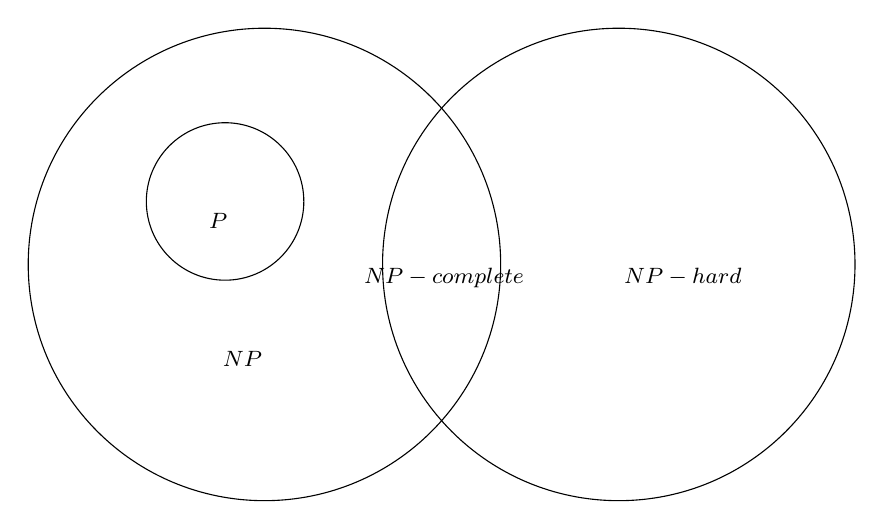
\begin{tikzpicture}
      \draw (0,2) circle (3cm);
      \put(-15,20){{\footnotesize $NP$}};
      \draw (4.5,2) circle (3cm);
      \put(130,50){{\footnotesize $NP-hard$}};
      \draw (-0.5,2.8) circle (1cm);
      \put(-20,70){{\footnotesize $P$}};
      \put(36,50){{\footnotesize $NP-complete$}};
	\end{tikzpicture}
	\caption{P, NP, NP-hard og NP-complete.}
	\label{fig.dijkstraexmp}
\end{figure}

Hvis vi kigger på Dijkstras algoritme i \autoref{kap:dijkstras}, ser vi, at denne algoritme løser problemer af typen P. Problemerne løses af en deterministisk algoritme i polynomisk tid, da grafen i et korteste vej-problem har optimal substruktur.

Dijkstras algoritme løser korteste vej-problemer, men ønsker vi at finde den længste vej igennem en orienteret ikke-cyklisk graf, er dette også et P problem. Havde grafen fx været ikke-orienteret og cyklisk, havde det været et NP-complete problem, men beviset udelades. Vigtigt at notere er blot, at disse ikke kan løses af en deterministisk algoritme, da grafen i disse længste vej-problemer ikke har optimal substruktur.
I Eksempel \ref{exmp.np} ses det, hvordan substrukturen i en ikke-orienteret, cyklisk graf er, for henholdsvis korteste og længste vej-problemer.

\begin{exmp} \label{exmp.np}
På \autoref{fig:laengste.vej} ses det, at den korteste vej  fra $v_1$ til $v_4$ går igennem punktet $v_2$. Den korteste vej har optimal substruktur, hvilket ses ved, at den korteste vej fra $v_{1}$ til $v_{4}$, $P_{1,2,4}=(v_{1},v_{2},v_{4})$, består af den korteste vej fra $v_{1}$ til $v_{2}$ og den korteste vej fra $v_{2}$ til $v_{4}$. 

Vi ser nu på den længste vej fra $v_1$ til $v_4$, $P_{1,2,4}=(v_{1},v_{2},v_{4})$ Hvis der havde været optimal substruktur, havde den længste vej, $P_{1,2,4}$, bestået af den længste vej fra $v_{1}$ til $v_{2}$ og den længste vej fra $v_{2}$ til $v_{4}$, men dette er ikke tilfældet. Den længste vej igennem grafen fra $v_{1}$ til $v_{2}$ er nemlig $P_{1,3,4,2}=(v_{1},v_{3},v_{4},v_{2})$, og den længste vej igennem grafen fra $v_{2}$ til $v_{4}$ er $P_{2,1,3,4}=(v_{2},v_{1},v_{3},v_{4})$. 




\begin{figure}[H]
\centering
	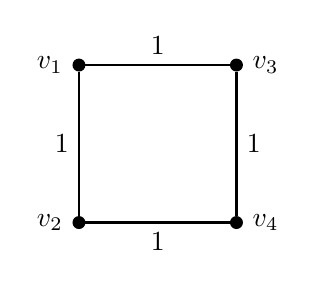
\begin{tikzpicture}
      \tikzset{enclosed/.style={draw, circle, inner sep=0pt, minimum size=.15cm, fill=black}}
%% Vertices
	%ikke orienteret
      	\node[enclosed, label={left, above: $v_1$}] (v1) at (0,2) {};
     	\node[enclosed, label={left, below: $v_2$}] (v2) at (0,0) {};
     	\node[enclosed, label={right, above: $v_3$}] (v3) at (2,2) {};
     	\node[enclosed, label={right, below: $v_4$}] (v4) at (2,0) {};    	
%Edges
	%Ikke orientered
		\path [thick] (v1) edge node[midway, left] {1} (v2);
		\path [thick] (v1) edge node[midway, above] {1} (v3);
		\path [thick] (v2) edge node[midway, below] {1} (v4);
		\path [thick] (v3) edge node[midway, right] {1} (v4);

\end{tikzpicture}
	\caption{Simpel vægtet graf.}
	\label{fig:laengste.vej}
\end{figure}

\end{exmp}


